\documentclass[12pt]{article}
\input{preamble}

\title{Working notes}
\author{Corey Jones, Scott Morrison, David Penneys}


\begin{document}
\maketitle


We define a truncated tensor product $\boxtimes$ of ATLJ modules, which is the usual tensor product, modulo the relations that
any closed diagram passes through a string, and
the $2\pi$ rotation acts identically.

Observe that if $V$ and $W$ are sub-ATLJ modules of a evaluable planar algebra $\cP_\bullet$, the ATLJ homomorphism $V \otimes W \to \cP_\bullet$ descends to an ATLJ homomorphism $V \boxtimes W \to \cP_\bullet$, because the additional relations we impose in the truncated tensor product automatically hold in an evaluable planar algebra.

We now aim to completely describe the decomposition of this truncated tensor product into irreducibles. 
To prepare for this, we need some discussion of lowest weight vectors in ATLJ modules.

Recall the isomorphism classes of minimal idempotents in the Temperley-Lieb-Jones algebra are the Jones-Wenzl idempotents $f^{(n)}$. 
It is convenient to pass to the idempotent completion, and consider the TLJ algebra as a semisimple category with simple objects $f^{(n)}$. 
The annular Temperley-Lieb-Jones category contains as a full subcategory the category with objects \nn{circle with one marked point, labelled by fn} which we call the tube category $\cT$. This inclusion is a Morita equivalence, giving an equivalence between $\Rep(ATLJ)$ and $\Rep(\cT)$. This is explained in \cite[Proposition 3.5]{1502.06543}.

\nn{Some remarks about what irreps of $\cT$ look like, and that there's only one annular consequence of the generator in each higher weight space.}

Suppose $\cV$ is some $\cT$ module.

\begin{lem}
When $\delta>2$, the lowest weight vectors in $\cV_m$ are the kernel of $\cL_m : \cV_m \to \cV_m$
$$
\cL_m = \mathfig{0.2}{LowestWeightTangle}.
$$
\end{lem}
\begin{proof}
First, it is clear that the lowest weight vectors are the kernel of $a$, where $$\mathfig{0.2}{LoweringOperator}.$$

Certainly $\ker(a)\subset\ker(\cL_m)$.
To show the other direction, we look at a basis of eigenvectors for $\cL_m$ acting on $\cV_m$ consisting of the new low weights, together with the annular consequences of previous low weights.  
$$
\mathfig{0.4}{PreviousLowWeightsInW}.
$$
By \cite[Proposition 5.3]{1502.06543}, as long as $\delta > 2$, $\cL_m$ has non-zero eigenvalue on the annular consequence.  Therefore only the uncappable vectors can be in the $Ker(\cL_m)$.
\end{proof}

We then define the two operators $\rho, \rho' : \cV_m \to \cV_m$ as
$$
\mathfig{0.3}{CutDownRotation}.
$$


\begin{lem}
The lowest weight vectors with rotational eigenvalue $\omega$ in $\cV_m$ can alternatively be characterized as the solutions of 
\begin{align*}
\rho(v) & = \omega v \\
\rho'(v) & = \omega^{-1} v.
\end{align*}
\end{lem}
\begin{proof}
First we expand the middle Jones-Wenzl idempotent in 
$$
\mathfig{0.3}{RhoRhoPrime}
$$
into a linear combination of Temperley-Lieb-Jones diagrams. 
Only the identity diagram and the diagram
$$
\mathfig{0.2}{JonesProjection}
$$
contribute, and we obtain
$
\rho \circ \rho' = \id_{W_m} - [m-1]/[m] \cL_m
$.
If $v$ is a eigenvector with eigenvalue $\omega$, then $$\rho \circ \rho'(v)=v-[m-1]/[m] \cL_m (v),$$ so $\cL_m(v)=0$, and $v$ is uncappable.
The converse is trivial.
\end{proof}


\begin{defn}
Consider irreducible $\cT$ modules $V^{n_+, \omega_+}$ and $V^{n_-, \omega_-}$, with lowest weight generators $S_+$ and $S_-$. (The use of $\pm$ as a label here has nothing to do with shadings; it's just convenient for our later formulas.) Fix $m\geq 0$ such that $n_+ + n_- + m = 0 \pmod 2$,
and define for $0 \leq i \leq \lfloor (m-2)/2 \rfloor$ and $0 \leq j < m - 2i$ 
\begin{align}
\label{eq:basis-elements}
T_{i,j} & = \mathfig{0.2}{Tij_generic}
\end{align}
where $k_i = (n_+ + n_- - m)/2 + i$. Here \nn{the squiggle lines just mean vertical strands.}
It will be helpful in what follows to consider $j \pmod{m-2i}$, because we are insisting that $2\pi$ rotations act trivially.

If $n_+ \neq n_-$ we need to properly interpret some special cases. We mean
\begin{align*}
T_{i,j} & = 
\begin{cases}
\mathfig{0.16}{Tij_right} & \text{when $n_- \leq k_i < n_+$, and} \\
\mathfig{0.16}{Tij_left} & \text{when $n_+ \leq k_i < n_-$.}
\end{cases}
\end{align*}
\end{defn}

\begin{fact}
A basis for $\left(V^{n_+, \omega_+} \boxtimes V^{n_-, \omega_-}\right)_m$ is given by $\{T_{i,j}\}$ for $0 \leq i \leq \lfloor (m-2)/2 \rfloor$ and $0 \leq i < m - 2i$.
\end{fact}

\begin{lem}
Consider irreducible $\cT$ modules $V^{n_+, \omega_+}$ and $V^{n_-, \omega_-}$, and let $U=V^{n_+, \omega_+} \boxtimes V^{n_-, \omega_-}$.
Let $W_m$ be the space of uncappable vectors in $U_m$.
Then $$\dim(W_m)=\begin{cases} m & \text{if $n_+ + n_- + m = 0 \pmod 2$, and} \\ 0 & \text{otherwise.}\end{cases}$$
\end{lem}
\begin{proof}
Let $\gA_m(S)$ be the space of $\cT$-annular consequences of $S$ in $U_m$.

Assume for now that $n_+ = n_- \pmod 2$, and that $m$ is even. \nn{The other case is similar.}
We use the basis for $U_m$ described above, to count dimensions.
It's now straightforward that $\dim(U_m)=m+\dim(U_{m-2})$, since
$$
U_{m}
=
\gA_m(W_0)\oplus\cdots\oplus \gA_m(W_{m-2})\oplus W_m 
= 
\gA_m(U_{m-2})\oplus W_m
$$
Note that $U_{2}=W_{2}$ since $W_{0}$ is the ``trivial'' representation. 
By induction on $m$, it suffices to show that $\dim(W_{2})=2$.  
This follows from direct computation.
\end{proof}

\nn{needs a home, or to be deleted:
\begin{itemize}
\item
if you shift $\star$ counterclockwise by one strand, multiply by $\sigma_S$ and switch $\check{}\,$:
$$
\begin{tikzpicture}[baseline = 0cm]
	\draw[thick, unshaded] (0,0) circle (1cm);
	\draw (0,0)--(-10:1cm);
	\draw (30:1cm) --(0,0); 
	\draw (0,0)--(70:1cm);
	\draw (110:1cm) --(0,0); 
	\draw (0,0)--(150:1cm);
	\draw (190:1cm) --(0,0); 
	\draw (0,0)--(230:1cm);
	\draw (310:1cm) --(0,0); 
	\draw[thick, unshaded] (0,0) circle (.4cm);
	\node at (90:.52) {$\star$};
	\node at (0,-.6) {$\cdots$};
	\node at (0,0) {$S$};
	\node at (90:.88) {$\star$};
\end{tikzpicture}
=
\sigma_S\,
\begin{tikzpicture}[baseline = 0cm]
	\draw[thick, unshaded] (0,0) circle (1cm);
	\draw (0,0)--(-10:1cm);
	\draw (30:1cm) --(0,0); 
	\draw (0,0)--(70:1cm);
	\draw (110:1cm) --(0,0); 
	\draw (0,0)--(150:1cm);
	\draw (190:1cm) --(0,0); 
	\draw (0,0)--(230:1cm);
	\draw (310:1cm) --(0,0); 
	\draw[thick, unshaded] (0,0) circle (.4cm);
	\node at (130:.52) {$\star$};
	\node at (0,-.6) {$\cdots$};
	\node at (0,0) {$\check{S}$};
	\node at (90:.88) {$\star$};
\end{tikzpicture}
$$
\item
if you shift $\star$ clockwise by one strand, multiply by $\sigma_S^{-1}$ and switch $\check{}\,$:
$$
\begin{tikzpicture}[baseline = 0cm]
	\draw[thick, unshaded] (0,0) circle (1cm);
	\draw (0,0)--(-10:1cm);
	\draw (30:1cm) --(0,0); 
	\draw (0,0)--(70:1cm);
	\draw (110:1cm) --(0,0); 
	\draw (0,0)--(150:1cm);
	\draw (190:1cm) --(0,0); 
	\draw (0,0)--(230:1cm);
	\draw (310:1cm) --(0,0); 
	\draw[thick, unshaded] (0,0) circle (.4cm);
	\node at (90:.52) {$\star$};
	\node at (0,-.6) {$\cdots$};
	\node at (0,0) {$S$};
	\node at (90:.88) {$\star$};
\end{tikzpicture}
=
\sigma_S^{-1}\,
\begin{tikzpicture}[baseline = 0cm]
	\draw[thick, unshaded] (0,0) circle (1cm);
	\draw (0,0)--(-10:1cm);
	\draw (30:1cm) --(0,0); 
	\draw (0,0)--(70:1cm);
	\draw (110:1cm) --(0,0); 
	\draw (0,0)--(150:1cm);
	\draw (190:1cm) --(0,0); 
	\draw (0,0)--(230:1cm);
	\draw (310:1cm) --(0,0); 
	\draw[thick, unshaded] (0,0) circle (.4cm);
	\node at (50:.52) {$\star$};
	\node at (0,-.6) {$\cdots$};
	\node at (0,0) {$\check{S}$};
	\node at (90:.88) {$\star$};
\end{tikzpicture}
$$
\end{itemize}
}

\begin{thm}
Consider irreducible $\cT$ modules $V^{n_+, \omega_+}$ and $V^{n_-, \omega_-}$, with lowest weight generators $S_+$ and $S_-$.
The truncated tensor product decomposes as
$$
V^{n_+, \omega_+} \boxtimes V^{n_-, \omega_-} 
\iso 
\bigoplus_{\substack{m \geq 0 \\ \text{$m + n_+  + n_-$ is even} \\ \omega^m = 1}} V^{m, \omega},
$$
with low weight generators 
$$
X_{m, \omega} 
= 
\sum_{i=0}^{\lfloor\frac{m-2}{2}\rfloor}
\left(X_{m,\omega}\right)_i
$$
with
\begin{align*}
\left(X_{m,\omega}\right)_0 & =  \sum_{j=0}^{m-1} \omega^{-j} T_{0,j} \\
\left(X_{m,\omega}\right)_{i+1} = - (\mu_{i+1} - \omega)^{-1} \nu_i \left(X_{m,\omega}\right)_i
\end{align*}
where $T_{i,j}$ is as defined in Equation \eqref{eq:basis-elements}, and the linear operators $\mu_i, \nu_i$ are as defined in the proof.
\end{thm}
\begin{proof}
We apply $\rho$ to $T_{i,j}$ and expand the lower Jones-Wenzl idempotent.
$$
\rho(T_{i,j})=
\mathfig{0.2}{RhoTij}
$$
Certainly the identity term contributes, and the only place we can put a cup on top is the top right.
Because the top right cup will result in an extra strand passing around the bottom of the diagram, no matter where we put a cap along the bottom of the expansion of the Jones-Wenzl idempotent, the total number of strands around the bottom cannot decrease. 
Thus the terms $T_{i',j'}$ which appear in $\rho(T_{i,j})$ can never have $i'<i$.

We first discuss the identity term in the expansion of the lower Jones-Wenzl idempotent. When $i > 0$, we end up with a cup attached to the upper Jones-Wenzl, giving zero. When $i=0$, we obtain $T_{0,j+1}$. We thus write this contribution as $\truth{i=0} T_{i, j+1}$, where here and below we use the notation $\truth{P} = 1$ if $P$ is true, $\truth{P} = 0$ otherwise.

In general there are four different places the cap could appear along the bottom edge of the Jones-Wenzl idempotent. Three of these are between an adjacent pair of the four multistrands connecting to the bottom edge of that idempotent. The fourth is within either the 2nd or 3rd multistrand, in the position so that it bridges between $S_+$ and $S_-$.
We can thus have
\begin{enumerate}[(a)]
\item
\label{item:purple}
\textcolor{purple}{
a cap appearing with $i-1$ strands to the left, between the first multistrand and the next,
}
\item
\label{item:orange}
\textcolor{orange}{
a cap appearing with $i+j-1$ strands to the left, between the second and third multstrands,
}
\item
\label{item:red}
\textcolor{red}{
a cap appearing with $m-i-1$ strands to the left, between the third and fourth multistrands, or
}
\item
\label{item:green}
\textcolor{DarkGreen}{
a `bridging' cap, which only occurs when $k_i \leq n_+, n_-$ (that is, the generators are not totally connected),
which either
\begin{itemize}
\item lies within the second multistrand, and appears with $i+j-n_-+k_i - 1$ strands to the left, or
\item lies within the third multistrand, and appears with $i+j+n_+-k_i -1$ strands to the left.
\end{itemize}
}
\end{enumerate}
%In general, the bridging cap appears with $i - 1 + (j+n_+-k_i \pmod{m-2i})$ strands to the left.
(The colour coding of these cases is used throughout the formulas below, to indicate terms arising from each of these possibilities.)

Note that if $i=0$, cases \eqref{item:purple} and \eqref{item:red} cannot occur, while if $j=0$ case \eqref{item:orange} cannot occur. Moreover, in case \eqref{item:purple} above we have been careful to say that the cap occurs between the first multistrand and \emph{the next} multistrand, because in special cases the next multistrand is not the second one. In particular, when $j=0$, the cap actually connects the first multistrand with the third, because the second is absent. The third multistrand, with $m-2i-j$ strands, is never absent, so this is the only special case of this type.

Finally, the bridging cap in case \eqref{item:green} occurs within the second multistrand exactly if $m-2i-j < n_+ - k_i$ or equivalently $i+j > (m - n_+ + n_-)/2$, and within the third multistrand exactly if $m-2i-j > n_+ - k_i$, or equivalently when $i+j < (m - n_+ + n_-)/2$. When equality occurs, we must remember to omit this case, because it is redundant with case \eqref{item:orange}, the cap between the second and third multistrands.

We now analyze the resulting diagram in each of the four cases, ignoring for now the coefficients arising in the Jones-Wenzl idempotent. As there is always a cup in the top right corner of the Temperley-Lieb diagram, there is an extra strand passing around the bottom of the diagram, thereby increasing $i$ by one.
\begin{enumerate}[(a)]
\item
\textcolor{purple}{
a cap between the first multistrand and the next has the effect of reducing both $i$ and $j$, in net producing $T_{i,j-1}$ (one needs to consider carefully that this is still true when $j=0$, that is, the second multistrand is absent; recall we consider $j \pmod{m-2i}$, because of $2\pi$ rotational invariance),
}
\item
\textcolor{orange}{
a cap between the second and third multistrands reduces $j$, producing $T_{i+1, j-1}$, except that the generators may have undergone a rotation: in the cases where the generators are not totally connected, we obtain $\sigma_+^{-1} \sigma_- T_{i+1, j-1}$, while when the generators are totally connected (i.e. $k_i \geq n_+$ or $k_i \geq   n_-$), we just obtain $T_{i+1,j-1}$,
}
\item
\textcolor{red}{
a cap between the third and fourth multistrands reduces $i$ but increases $j$, producing $T_{i, j+1}$, and finally
}
\item
\textcolor{DarkGreen}{
the bridging cap (when it is distinct from case \eqref{item:orange}) reduces $j$ by two when it lies within the second multistrand, producing $T_{i+1, j - 2}$, and does not change $j$ when it lies within the third multistrand, producing $T_{i+1, j}$. 
}
\end{enumerate}

In each of the cases above, we interpret $T_{i,j}$ as zero if $i$ becomes too large, that is $i > \lfloor (m-2)/2 \rfloor$. (This is of course justified by our having imposed that closed diagrams move freely, so the resulting $T_{i,j}$ has a Jones-Wenzl idempotent with cups attached to it.)

To compute the expansion of the Jones-Wenzl idempotent, we quickly recall
\begin{lem}
The coefficient of the following Temperley-Lieb diagram in the Jones-Wenzl idempotent $\jw{m}$ is given by
\begin{align*}
\underset{\in \jw{m}}{\textrm{coeff}}
\left(
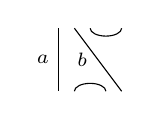
\begin{tikzpicture}[baseline = -.1cm, yscale=-.5]
	\draw (-.5,-.8)--(-.5,.8);
	\draw (-.3,.8) arc (-180:0:.2cm);
	\draw (-.3,-.8)--(.3,.8);
	\draw (-.1,-.8) arc (180:0:.2cm);
	\node at (-.7,0) {{\scriptsize{$a$}}};
	\node at (-.2,0) {{\scriptsize{$b$}}};
    \node at (.2,0) {$\phantom{c}$};
\end{tikzpicture}
\right)
& =
(-1)^{m-a+1}\frac{[a+1]}{[m]}.
\end{align*}
\end{lem}

  
Putting all this together, we obtain the formula
\begin{align*}
\rho(T_{i,j}) & =
\truth{i = 0} T_{i, j + 1} \\
& \qquad +
\truth{i \neq 0} \textcolor{purple}{(-1)^{m-i} [i][m]^{-1}} T_{i,j-1} \\
& \qquad +
\truth{j \neq 0}\textcolor{orange}{(-1)^{m-i-j} [i+j][m]^{-1}} \left(\sigma_+^{-1} \sigma_-\right)^{\truth{k_i \leq n_+} \truth{k_i \leq n_-}} T_{i+1, j-1} \\
& \qquad +
\truth{i \neq 0}\textcolor{red}{(-1)^{i}  [m-i][m]^{-1}} T_{i, j + 1} \\
& \qquad +
\truth{k_i \leq n_+} \truth{k_i \leq n_-}
\truth{i+j > (m - n_+ + n_-)/2} \times \\
& \qquad \quad \times \textcolor{DarkGreen}{(-1)^{(-m + n_+ - n_-)/2 + j} [2i + j + (-m + n_+ - n_-)/2][m]^{-1}} T_{i+1,j-2} \\
& \qquad +
\truth{k_i \leq n_+} \truth{k_i \leq n_-}
\truth{i+j < (m - n_+ + n_-)/2} \times \\
& \qquad \quad \times \textcolor{DarkGreen}{(-1)^{(m + n_+ - n_-)/2 + j} [j+ (m + n_+ - n_-)/2 ][m]^{-1}} T_{i+1,j}
\end{align*}

Happily, some simplifications occur here. In the second term, we can omit the $\truth{i\neq0}$ factor, since the quantum integer $[0]$ is zero. The first term (corresponding to the identity term in the expansion of the Jones-Wenzl idempotent) and the fourth term (corresponding to case \eqref{item:red}, a cap connecting the third and fourth multistrands) can be combined to give $(-1)^i [m-i][m]^{-1} T_{i,j+1}$. We have
\begin{align*}
\rho(T_{i,j}) & =
(-1)^i[m-i][m]^{-1} T_{i, j + 1} \\
& \qquad +
\textcolor{purple}{(-1)^{m-i} [i][m]^{-1}} T_{i,j-1} \\
& \qquad +
\truth{j \neq 0}\textcolor{orange}{(-1)^{m-i-j} [i+j][m]^{-1}} \left(\sigma_+^{-1} \sigma_-\right)^{\truth{k_i \leq n_+} \truth{k_i \leq n_-}} T_{i+1, j-1} \\
& \qquad +
\truth{k_i \leq n_+} \truth{k_i \leq n_-}
\truth{i+j > (m - n_+ + n_-)/2} \times \\
& \qquad \quad \times \textcolor{DarkGreen}{(-1)^{(-m + n_+ - n_-)/2 + j} [2i + j + (-m + n_+ - n_-)/2][m]^{-1}} T_{i+1,j-2} \\
& \qquad +
\truth{k_i \leq n_+} \truth{k_i \leq n_-}
\truth{i+j < (m - n_+ + n_-)/2} \times \\
& \qquad \quad \times \textcolor{DarkGreen}{(-1)^{(m + n_+ - n_-)/2 + j} [j+ (m + n_+ - n_-)/2 ][m]^{-1}} T_{i+1,j}
\end{align*}


Writing $\cT_i = \Span \{ T_{i,j} \}_{0 \leq j < m- 2i}$, we can write $\rho \mid_{\cT_i} = \mu_i + \nu_i$, where
\begin{align*}
\mu_i :  \cT_i & \to \cT_i \\
  T_{i,j} & \mapsto (-1)^i [m]^{-1} \left( [m-i] T_{i,j+1} + (-1)^{m}[i] T_{i,j-1}\right) \\
\intertext{and}
\nu_i : \cT_i & \to \cT_{i+1}.
\end{align*}
Thus any eigenvector $\rho(X) = \omega X$ is of the form $X = \sum_i X_i$, where for some $i_0$, $X_i = 0$ for $i < i_0$, and $\mu_{i_0} X_{i_0} = \omega X_{i_0}$.

In fact, $\mu_i$ is just a circulant matrix in this basis, and so has multiplicity free eigenvalues
$$\lambda_r = (-1)^i[m]^{-1} \left([m-i] \zeta_{m-2i}^{-r} + (-1)^{m}[i] \zeta_{m-2i}^r\right),$$
where $\zeta_{m-2i}$ is a primitive $(m-2i)$-th root of unity, with corresponding eigenvectors
$$v_r = \left(1, \zeta_{m-2i}^r , \zeta_{m-2i}^{2r} , \ldots, \zeta_{m-2i}^{(m-2i-1)r} \right).$$

Clearly when $i = 0$, these eigenvalues are exactly the $m$-th roots of unity, each with multiplicity one.
If $i > 0$, we claim that $\lambda_{r}$ is never an $m$-th root of unity; in fact they always have absolute value less than 1:
\begin{align*}
\lambda_{r} \overline{\lambda}_{r} 
 & = [m]^{-2}\left([m-i]^{2}+(-1)^{m}[m-i][i]\left(\zeta_{m-2i}^{-2r}+\zeta_{m-2i}^{2r}\right)+[i]^{2}\right) \\ 
 & \le [m]^{-2}\left([m-i]+[i]\right)^{2} \\
 & < 1
\end{align*}
(as always, we assume $q>1$, so we have the inequality $[a] + [b] < [a+b]$ for $a,b>0$).


Thus an eigenvector $\rho(X) = \omega X$ must have eigenvalue $\omega  = \zeta_m^r$ for some $r$, and in fact be of the form $X = \sum_i X_i$, for $X_i \in \cT_i$, with $X_0 = \sum_{j=0}^{m-1} \zeta^{-rj} T_{i,j}$. The eigenvector equation then becomes $\mu_{i+1} X_{i+1} + \nu_i X_i = \omega X_{i+1}$, which we may invert to obtain $X_{i+1} = - (\mu_{i+1} - \zeta_m^r)^{-1} \nu_i X_i$.

We thus have a unique solution to $\rho(X) = \zeta_m^r X$ for each $r$, given by $X = \sum_{i=0}^{\lfloor(m-2)/2\rfloor} X_i$, with
\begin{align*}
X_0 & = \sum_{j=0}^{m-1} \zeta^{-rj} T_{0,j} \\
\intertext{and}
X_{i+1} & = - (\mu_{i+1} - \zeta_m^r)^{-1} \nu_i X_i.
\qedhere
\end{align*}
\end{proof}

\nn{Can we find the formulas for $\rho'$ just using the reflection in a vertical line?}

\nn{Can we sanity check the above formulas by finding eigenvectors separately for $\rho$ and for $\rho'$, and verifying they agree?}

\nn{Can we make more explicit formulas for $X_{>0}$?}


\begin{lem}
\label{lem:nu0}
When $n_+ = n_- = 2n$, we have
\begin{align*}
\nu_i(T_{i,j})
& = (-1)^j[m]^{-1} \times\\
& \quad \Bigg(
\truth{j \neq 0}(-1)^{m-i} [i+j] \left(\sigma_+^{-1} \sigma_-\right) T_{i+1, j-1} \\
& \qquad +
\truth{i+j > m/2} [2i + j + -m/2] T_{i+1,j-2} \\
& \qquad +
\truth{i+j < m/2} [j+ m/2 ] T_{i+1,j} \Bigg)
\end{align*}
and
\begin{align*}
\nu_0(T_{0,j})
& = (-1)^j [m]^{-1} \times \\
& \quad \Bigg(
(-1)^{m} [j] \left(\sigma_+^{-1} \sigma_-\right) T_{1, j-1} \\
& \qquad + \truth{j > m/2} [j- m/2] T_{1,j - 2} \\
& \qquad + \truth{j < m/2} [j+ m/2] T_{1,j} \Bigg).
\end{align*}
\end{lem}

\begin{lem}
The resolvent of $\mu_i$ is given by
\begin{align*}
(\mu_i - z)^{-1}(T_{i,j}) & = ???
\end{align*}
\end{lem}
\begin{proof}
The eigenvectors described above for $\mu_i$ are orthogonal, so we can diagonalize:
\begin{align*}
\mu_i = P D P'
\end{align*}
where $D$ is diagonal with 
$D_{\ell\ell} = (-1)^i(m-2i)^{-1}[m]^{-1} \left([m-i] \zeta_{m-2i}^{-\ell} + (-1)^{m}[i] \zeta_{m-2i}^\ell\right)$, 
$P_{jj'} = \zeta_{m-2i}^{jj'}$, and 
$P'_{jj'} = \zeta_{m-2i}^{-jj'}$.
We obtain
\begin{align*}
(\mu_i - z)^{-1}_{jj'} & = (-1)^i(m-2i)^{-1}[m]^{-1} \sum_{\ell} \zeta_{m-2i}^{\ell(j-j')}  \left([m-i] \zeta_{m-2i}^{-\ell} + (-1)^{m}[i] \zeta_{m-2i}^\ell - z\right)^{-1} \\
...
\end{align*}
\nn{which I can't think of anything to do with...}
\end{proof}

We now consider $V$ an irreducible ATLJ submodule of some planar algebra $P$, and the ATLJ homomorphism $\psi: V\boxtimes V\rightarrow P$. Let $S$ denote a lowest weight generator of $V$, with weight $2n$ and rotational eigenvalue $\sigma$.

For $\omega$ a $(2n+2)$-th root of unity, we have the unique (up to scale) lowest weight vector $X_\omega = \sum X_{\omega,i}$ in $(V \boxtimes V)_{2n+2}$ with rotational eigenvalue $\omega$ with
\begin{align*}
X_{\omega,0} & = \sum_{j=0}^{2n+1} \omega^{-j} T_{0,j} \\
X_{\omega,i+1} & = - (\mu_{i+1} - \omega)^{-1} \nu_i X_i \\
\intertext{and in particular, by Lemma \ref{lem:nu0}}
X_{\omega,1} & = - (\mu_{i+1} - \omega)^{-1}  ...
\end{align*}

\textbf{Super Transitivity obstruction????} It seems like our above work should yield $*^{n-1}1$ obstructions (no zeros), and in fact it looks like (preliminarily) we get $2n+2$ of them! (I think half are redundant since the two generators are equal in our planar algebra).

The idea is as follows:

Let $\omega$ be a $2n+2^{th}$ root of unity, and let $X=\sum X_{i}$ be the eigenvector in $V\boxtimes V$ as above, where $m=2n+2$. Let $\psi: V\boxtimes V\rightarrow P$ be the planar algebra map.  By n-1 super transitivity, we know that $\psi(X_i)=0$ for $i>1$, and so we have that $\psi(X)=\psi(X_1)+\psi(X_0)$.  Let $R$ be the picture with $f_{2n+2}$ and top and an $\check{S}$ attached with a single strand around the back (1-strand box-jellyfish I think you call it?).  From planar algebra theory, we know that $\psi(X_1)=a_{\omega, \sigma, r, \check{r}} R$, where $r\ (\text{resp.}\ \check{r})$ appears in the quadratic relation of $S\ (\text{resp.}\ \check{S})$, and $a_{\omega, \sigma, r, \check{r}}$ (to be computed). (Note, in the subfactor case the appearance of $r$ and $\check{r}$ in the various terms depends on the parity of $j$.  If $r=\check{r}$, then it appears multiplicatively, and we can factor it out so that $a_{\omega, \sigma, r, \check{r}}$ is $r$ times something depending only on $\omega$ and $\sigma$, but in general, this number will also depend on $r$ and $\check{r}$.) If $\psi(X)$ is $0$, then $R^{*}\psi(X)=0$, and we can evaluate this in the planar algebra to get an equation with just numbers, involving quantum numbers, $\sigma$, $r$ and $\omega$ (and $\check{r}$ in the subfactor case!)  If $\psi(X)$ is not $0$, then it is an eigenvector of rotation, so is orthogonal to annular consequences of lower stuff (in particular of $\check{S}$), and thus we still have $R^{*}\psi(X)=0$!  Thus we get the same equation, independently of the annular multiplicities of the n+1 box space!  The number of such equations is 2n+2 (but we will see that only half of them are new.)


Could this give us supertransitivity obstructions, or are the above equations  $0=0$?  It seems unlikely from a preliminary investigation that we always (or ever) get $0=0$.

\bigskip

Lets do a computation,  in particular lets compute $R^{*}\psi(X_0)$.  First, we assume now we are in spherical subfactor-shaded land, (although it appears we get a much stronger obstruction for spherical non-shaded, as to be expected).  Then we have three parameters: $r_{0}:=r=Tr(S^{3})$,  $r_{1}:=\check{r}=Tr(\check{S}^{3})$, and $\sigma$. For $0\le j\le n$, we have

$$R^{*}\psi(T_{0,j})=(-1)^{j}\sigma^{j}\frac{[2n+2-j]}{[2n+2]} r_{j\ \text{mod}2}+(-1)^{n+j+1}\sigma^{j+1}\frac{[n+1-j]}{[2n+2]} r_{(j+1)\text{mod}2}$$
$$+(-1)^{j}\sigma^{j-2}\frac{[j]}{[2n+2]} r_{j\ \text{mod}2}+(-1)^{n+j+1}\sigma^{j-1}\frac{[n+1+j]}{[2n+2]} r_{(j+1)\text{mod}2}$$

Even though there are special cases in the pictures, interpreting $[0]=0$ in fact leads to the above formula for all cases!  Now, recall that for a $2n+2$ root of unity $\omega$, $X_{0}=\sum^{2n+1}_{j=0} \omega^{-j}T_{0,j}$.  Furthermore, since $\sigma$ is a $2n^{th}$ root of unity, we see that $\psi(T_{0,j})=\psi(T_{0,j-n-1})$ for $j\ge n+1$.

Thus 

$$R^{*}\psi(X_0)=\sum^{n}_{j=0}(\omega^{-j}+\omega^{-j+n+1})\left[ \left(\sigma^{j}\frac{[2n+2-j]}{[2n+2]}
+\sigma^{j-2}\frac{[j]}{[2n+2]}\right)(-1)^{j} r_{j\ \text{mod}2}
\right.$$


$$\left.+\left( \sigma^{j+1}\frac{[n+1-j]}{[2n+2]}+\sigma^{j-1}\frac{[n+1+j]}{[2n+2]} \right)(-1)^{n+j+1}r_{(j+1)\text{mod}2}\right]$$

\nn{All these formulas need to be checked, include pictures}

We also note that the above formula is entirely general, and requires no assumption on super-transitivity.  It is the computation of $a_{\omega, \sigma}$ that depends on super transitivity

Now, to obtain our equation depending on $\omega$, we have

$$0=a_{\omega, \sigma, r, \check{r}} R^{*}R+R^{*}\psi(X_0)$$
$$= a_{\omega, \sigma, r, \check{r}}([2n+2]^{-1}(q^{2n+2}+q^{-2n-2}-\sigma^{2}-\sigma^{-2}))$$
$$
+\sum^{n}_{j=0}(\omega^{-j}+\omega^{-j+n+1})\left[ \left(\sigma^{j}\frac{[2n+2-j]}{[2n+2]}
+\sigma^{j-2}\frac{[j]}{[2n+2]}\right)(-1)^{j} r_{j\ \text{mod}2}
\right.$$


$$\left.+\left( \sigma^{j+1}\frac{[n+1-j]}{[2n+2]}+\sigma^{j-1}\frac{[n+1+j]}{[2n+2]} \right)(-1)^{n+j+1}r_{(j+1)\text{mod}2}\right]$$

Notice that exchanging $\omega$ with $\omega^{n+1}$ gives the same equation, and since $\omega$ is a $2n+2$ root of unity, we really only have $n+1$ equations.

\nn{IMPORTANT:} We want to point out an interesting feature of the above equations:  If $r=\check{r}$ (so in particular for unshaded planar algebras), we can factor $r$ out and divide by it.  In this case, for each $\omega$ the above equation depends only on $q$, $\sigma$ and $n$.  This seems quite remarkable.  Can we plug it into mathematica, and see what happens?





\hrule

\bigskip

\nn{some old stuff has been moved to obsolete/obsolete.tex}

\nn{old stuff}



Now suppose $S$ comes from an initial triple point, and we have *10 annular multiplicity sequence.

Consequences:
Notice $\mu(T_{j,i})=0$ for $j>1$, because $P$ is $(n-1)$-supertransitive. 
 By $*10$ assumption, $\mu(X_{\omega})=0$.
If $S^{2}= r S + TLJ$, then $\mu(T_{1,i})=r \sigma^{i}$ (box 1-strand jellyfish).

From formula for $c^{\omega}_{j,i},\ c_{0,i}=\omega^{i} c^{\omega}_{0,0}$, and we can pick $c^{\omega}_{0,0} = 1$.

$\sum_{\omega} \mu(X_{\omega})=0$.
We could worry about the diagrams $\mu(T_{0,i})$, but these appear in $\mu(X_{\omega})$ with coefficient $c_{0,i}=\omega^{i}$.


Note, that for $i \neq 0 \pmod{2n+2}$, $\sum_{\omega} \omega^{i}=0$.

\begin{align*}
0 & = \sum_{\omega} \mu(X_{\omega}) \\
   & = \sum_{\omega, i} c^{\omega}_{0,i} \mu(T_{0,i}) + c^{\omega}_{1,i} \mu(T_{1,i}) \\
   & = \sum_i \left( \left(\sum_\omega \omega^i\right) \mu(T_{0,i}) + \sum_\omega c^{\omega}_{1,i} \mu(T_{1,i})\right) \\
   & = (2n+2) \mu(T_{0,0}) + r \left(\sum_i \left(\sum_\omega c^{\omega}_{1,i}\right) \sigma^{i}\right) (box 1-strand jellyfish)
\end{align*}

The upshot is that we have an equation:
$$
\mathfig{0.2}{QuadraticEqn.jpg}
$$

Step 1: Let's assume there’s some constant $Q$ for the (?) above, and calculate a formula in terms of $Q$. 
\begin{itemize}
\item
Let's expand the $(2n+2)$-strand JW, but not all the way, and equate coefficients of certain diagrams.
\item
We're interested in calculating the coefficients on both sides of the following diagram:
$$
\mathfig{0.12}{SCupTopLeft.jpg}
$$
\item
On the left hand side, there’s only 2 diagrams we need the coefficients for:
$$
\mathfig{0.2}{JWCupTopLeft.jpg}
$$
The first is $-[2n+1]/[2n+2]$ and the second $(-1)^{2n+1}/[2n+2]$

\end{itemize}


\todo{look at the alternating sum $\sum_{k=0}^{2n+1} (-1)^{k} \mu(X_{\zeta^{k}})$, where $\zeta = \exp(2\pi i / 2n+2)$}

\renewcommand*{\bibfont}{\small}
\setlength{\bibitemsep}{0pt}
\raggedright
\printbibliography
\end{document}
